\begin{figure}[!h]
	\begin{center}
		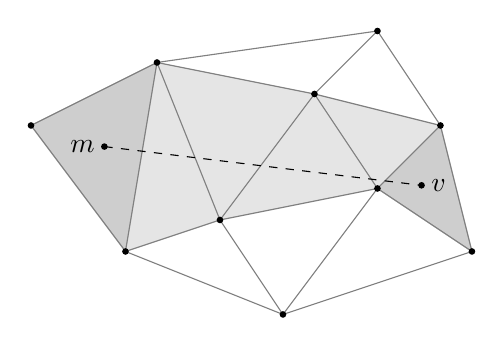
\begin{tikzpicture}[scale=0.4]
		%\draw [<->,thick] (0,10) node (yaxis) [left] {}
		%|- (15,0) node (xaxis) [below] {};
		
		\filldraw[fill=black, opacity=0.1] 	(2,7) -- (6,9) -- 
											(11,8) -- (15,7) -- 
											(16,3) -- (13,5) --
											(8,4) -- (5,3) --
											cycle;
		
		\filldraw[fill=black, opacity=0.1] 	(2,7) -- (6,9) -- (5,3) --
											cycle;
											
		\filldraw[fill=black, opacity=0.1] 	(15,7) -- (13,5) -- (16,3) --
													cycle;
		
		
		
		\draw [-,gray] ( 2,7) -- ( 6,9);
		\draw [-,gray] ( 6,9) -- ( 5,3);
		\draw [-,gray] ( 5,3) -- ( 2,7);
		\draw [-,gray] ( 6,9) -- ( 8,4);
		\draw [-,gray] (10,1) -- ( 8,4);
		\draw [-,gray] ( 5,3) -- (10,1);
		\draw [-,gray] ( 8,4) -- ( 5,3);
		\draw [-,gray] ( 8,4) -- (11,8);
		\draw [-,gray] (11,8) -- (6,9);
		\draw [-,gray] ( 6,9) -- (13,10);
		\draw [-,gray] (11,8) -- (13,10);
		\draw [-,gray] (15,7) -- (13,10);
		\draw [-,gray] (16,3) -- (15,7);
		\draw [-,gray] (16,3) -- (10,1);
		\draw [-,gray] (16,3) -- (13,5);
		\draw [-,gray] (13,5) -- (15,7);
		\draw [-,gray] (13,5) -- (10,1);
		\draw [-,gray] (13,5) -- (8,4);
		\draw [-,gray] (13,5) -- (11,8);
		\draw [-,gray] (15,7) -- (11,8);
		
		
		%centroids
		\fill ( 2, 7) circle (3pt);
		\fill ( 5, 3) circle (3pt);
		\fill ( 6, 9) circle (3pt);
		\fill ( 8, 4) circle (3pt);
		\fill (10, 1) circle (3pt);
		\fill (11, 8) circle (3pt);
		\fill (13, 5) circle (3pt);
		\fill (13,10) circle (3pt);
		\fill (15, 7) circle (3pt);
		\fill (16, 3) circle (3pt);
		
		
		\draw [-,dashed]( 4.33,6.33) -- ( 14.4, 5.1);
		%\draw []( 2,7) -- node[anchor=south]{$t$} ( 6,9);
		\fill ( 4.33,6.33) circle (3pt) node[anchor=east]{$m$};
		\fill (14.4, 5.1) circle (3pt) node[anchor=west]{$v$};
		\end{tikzpicture}
	\end{center}
	\caption{Illustration of the Walking Algorithm}
	\label{fig:wk1}
\end{figure}